\documentclass{article}
\usepackage{fancyhdr}
\usepackage{graphicx}
\usepackage{amssymb}
\usepackage{epstopdf}
\usepackage{amsmath}
%\usepackage{nicefrac}
\usepackage{amssymb}
%\usepackage{cite}
\usepackage{multirow}
%\usepackage{wrapfig}
%\usepackage{subfigure}
%\usepackage{todonotes}
\usepackage{listings}
\usepackage[utf8]{inputenc}
\usepackage[swedish]{babel} 
\usepackage[swedish]{cleveref}
\usepackage[retainorgcmds]{IEEEtrantools}
%\DeclareGraphicsRule{.tif}{png}{.png}{`convert #1 `dirname #1`/`basename #1 .tif`.png}
\graphicspath{{figures/}}
\numberwithin{equation}{section}

\title{F0047T\\Laboration: Spektrallinjer}
\author{Daniel Brolin, danbro-3@student.ltu.se \and Kenny Eriksson, keneri-3@student.ltu.se}

\begin{document}
\pagenumbering{gobble}
\maketitle
\newpage

\begin{abstract}
Frank-Hertz experiment var $1914$ det första elektriska mätningarna att tydligt visa kvantnaturen av atomer och ge inblick i deras kvantenerginivåer. Frank-Hertz experimentet vi utför accelererar elektroner genom ett moln av upphettad kvicksilvergas och mäter strömmen för olika spänningar och observerar det emmiterade ljuset från röret.

I mätningar kommer vi fram till en kvantspänningsskillnad på $\Delta U_A = 4.0~\textrm{eV}$ mellan miniman, se \cref{tab:maxmin}; vilket beräknas till en våglängd på $302~\textrm{nm}$, se \cref{eq:resultat}. Detta bör resultera i ett ljus, ej synligt med bara ögon, nästan ultraviolet ljus. I själva verket lös röret med ett ljus närmare turkos, vilket bör ligga någonstans i det blå spektrat mellan $450 - 495~\textrm{nm}$ vilket bör ge en spänning på $\approx 2.76~\textrm{eV}$.

Enligt fler källor, däribland en rapport från Manchester University\cite{bmfrankhertz} rapporterar kvantnivåer på $4.9~\textrm{V}$, vilket bör resultera i en rimligare och mer passande våglängd för det observerade skenet. $302~\textrm{nm}$ är väldigt nära den andra förväntade våglängden på $297~\textrm{nm}\cite{fhbook}$. 

Trots avvikelsen från de ``korrekta'' värdena har syftet med utförandet varit tydligt och förståelsen är densamma. Möjliga fel diskuteras i \cref{sec:disc}.
\end{abstract}
\newpage

% \tableofcontents % Sätt in när resten är klart och fixa eventuella problem då.
% \newpage

\pagenumbering{arabic}
\setcounter{page}{1}

\section{Introduktion}
\subsection*{Syfte}
Syftet med laborationen är att stifta bekantskap med relationen mellan det utstrålade ljuset från exciterade ämnen och energinivån hos de exciterade atomerna.
\subsubsection*{Frågeställningar:}
\begin{itemize}
	\item Räkna ut ett värde på Rydbergs konstant $R_H$ för väte
    \item Räkna ut ett värde på Rydbergs konstant $R_{Hg}$ för kvicksilver
\end{itemize}

\subsection*{Metod}
För att få ljus av just ett ämnes spektrum användes dels en vätgaslampa, dels en kvicksilverlampa. Dessa riktades in ett spektroskop i vilket det infallande ljuset spreds av ett gitter varvid våglängden av det infallande ljuset kan avgöras genom hur mycket det bryts.

\subsection*{Teori}
\subsubsection*{Brytning i gitter:}
När ljus av våglängd $\lambda$ träffar ett gitter med spaltavstånd $d$ i infallsvinkel $\theta_i$ kommer sambandet 
\begin{equation}
	d\left(\sin\theta_o-\sin\theta_i\right)=k\lambda: \quad k\in\mathbb{Z}
    \label{eq_gitterbrytning}
\end{equation}
där $\theta_o$ är den utgående vinkeln.

\subsubsection*{Rydbergs formel:}
När en atom går från ett exciterat tillstånd till ett lägre avges en foton med energin $E_{foton}=E_f-E_i$ där $E_f$ är energin av det slutgiltiga tillståndet och $E_i$ det initiala tillståndet. Fotonen kommer ha en våglängd $\lambda$ enligt Rydbergs formel:
\begin{equation}
	\frac{1}{\lambda}=R\left(\frac{1}{n^2}-\frac{1}{m^2}\right)
    \label{eq_Rydbergs_formel}
\end{equation}
där $n$ är det huvudkvanttalet för det initiala tillståndet $m$ är huvudkvanttalet för det slutgiltiga tillståndet, och $R$ är Rydbergs konstant beroende på vilket material som avger fotonen.
\newpage

\section{Resultat}
\subsection*{Vätgaslampa}
Experimentet ställdes upp enligt beskrivning, varpå tre linjer kunde ses genom spektroskopet. När de uppmätta utgångsvinklarna sätts in i \cref{eq_gitterbrytning}, $k$ sätts till $\pm1$ ($\pm{}$ ty mätningar gjordes för både positiva och negativa vinklar för ökad precision) och $\theta_i=0$ fås \cref{tb_expres_1}; \cref{tb_expres_2} fås då när de värdena sätts in i \cref{eq_gitterbrytning}
\begin{table}[!hb]
	\caption{Experimentellt resultat av mätningar på vätgaslampa. $\theta_j$ är genomsnittet av de två uppmätta vinklarna och den vinkel som används för fortsatta uträkningar.}
	\label{tb_expres_1}
    \begin{center}
    	\renewcommand{\arraystretch}{1.2}
		\begin{tabular}{| c | c | c | c |}
        	\hline
			 & $\theta_{+j}$ & $\theta_{-j}$ & $\theta_{j}$ \\
            \hline
            $\theta_{1}$ & $23.0^\circ$ & $-24.0^\circ$ & $23.5^\circ$ \\
            \hline
            $\theta_{2}$ & $16.75^\circ$ & $-17.75^\circ$ & $17.25^\circ$ \\
            \hline
            $\theta_{3}$ & $14.75^\circ$ & $-15.75^\circ$ & $15.25^\circ$ \\
            \hline
		\end{tabular}
	\end{center}
\end{table}
\begin{table}[!hb]
	\caption{Resulterande experimentell våglängd}
    \label{tb_expres_2}
    \begin{center}
    	\renewcommand{\arraystretch}{1.2}
		\begin{tabular}{| c | c |}
        	\hline
            $\lambda_1$ & $6.6458*10^{-7}$ m \\
            \hline
            $\lambda_2$ & $4.9424*10^{-7}$ m \\
            \hline
            $\lambda_3$ & $4.3839*10^{-7}$ m \\
            \hline
		\end{tabular}
	\end{center}
\end{table}

Enligt \cref{eq_Rydbergs_formel} ger större $m$ mindre $\lambda$ och mindre $\lambda$ i \cref{eq_gitterbrytning} ger mindre $\theta_o$, d.v.s. större $m$ svarar mot mindre $\theta_j$ i enlighet med \cref{tb_expres_1,tb_expres_2}. Det antas att alla språng slutar i det givna grundtillståndet $n=2$ enligt instruktion från labhandledning. 

Från \cref{eq_Rydbergs_formel} fås då tillsammans ovanstående att 
\begin{equation}
	\frac{1}{\lambda_j}=R_H\left(\frac{1}{4}-\frac{1}{(m+j-1)^2}\right)
    \label{eq_lambda_j_1}
\end{equation}
Härifrån definieras $\lambda_j$ för de tre mätvärdena:

\begin{IEEEeqnarray}{r C c}
	\lambda_1 & = & \frac{4}{R_H}\frac{m^2}{(m-2)(m+2)} \nonumber\\
    \lambda_2 & = & \frac{4}{R_H}\frac{(m+1)^2}{(m-1)(m+3)} \IEEEyesnumber\label{eq_lambda(m)_def} \\
    \lambda_3 & = & \frac{4}{R_H}\frac{(m+2)^2}{m(m+4)} \nonumber
\end{IEEEeqnarray}
varpå variablen $F_{ij}(m)$ samt konstanten $\lambda_{ij}$ definieras som 
\begin{equation}
	F_{ij}(m)=\frac{\lambda_i}{\lambda_j}=\lambda_{ij}
    \label{eq_F_def}
\end{equation}
där $F$ kommer från definitionerna i ekvation \ref{eq_lambda(m)_def} medan $\lambda_{ij}$ skapas från de experimentella värdena vilket ger \cref{tb_F_lambda_def}:
\begin{table}[!hb]
	\caption{$F_{ij}(m)$ och $\lambda_{ij}$ tabellerat. Eftersom $F$ för alla $ij$ innehåller den obekanta $4/R_H$ försvinner den vid division vilket låter $m$ räknas ut.} 
    \label{tb_F_lambda_def}
    \begin{center}
    	\renewcommand{\arraystretch}{1.7}
		\begin{tabular}{| c | c c c |}
			\hline
            $ij$ & $F_{ij}(m)$ & = & $\lambda_{ij}$ \\
            \hline
            32 & $\frac{m^2(m-1)(m+3)}{(m+1)^2(m-2)(m+2)}$ & = & 1.3447 \\
            \hline
            31 & $\frac{m^3(m+4)}{(m-2)(m+2)^3}$ & = & 1.5160 \\
            \hline
            21 & $\frac{m(m+1)^2(m+4)}{(m-1)(m+2)^2(m+3)}$ & = & 1.1274 \\
            \hline
		\end{tabular}
	\end{center}
\end{table}

Eftersom $F_{ij}(m)=\lambda_{ij}$ kommer det finnas ett gemensamt $m$ för vilket alla $F_{ij}(m)-\lambda_{ij}=0$, som fås grafiskt till 3:
\begin{figure}[htb]
	\begin{center}
		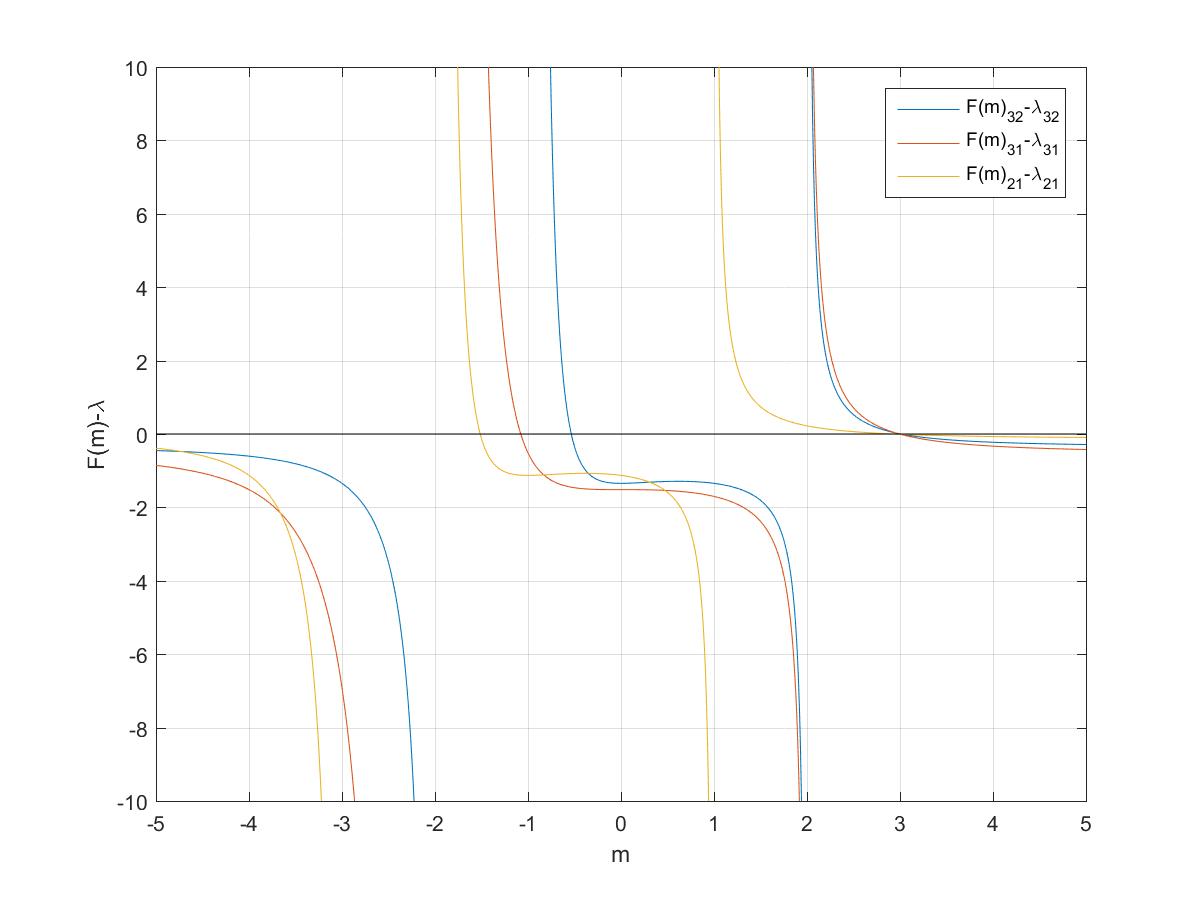
\includegraphics[width=9cm]{Finding_m.png}
        \caption{Enligt figuren passerar alla tre kurvor tillsammans genom 0 nära 3; specifikt 3.011, 2.994 och 2.930 vilket ger medelvärde 2.9783.}
	\end{center}
\end{figure}

När $m=3$ är känt sätts detta tillsammans med  de experimentella våglängderna in i \cref{eq_lambda_j_1} och $R_H$ bryts ut vilket ger \cref{tb_R_H}.
\begin{table}[htb]
	\caption{Numerisk uträkning av $R_H$ från experimentella värden.}
    \label{tb_R_H}
    \begin{center}
    \renewcommand{\arraystretch}{1.3}
		\begin{tabular}{| c c c c c |}
			\hline
            \rule{0pt}{3ex}$R_H(\lambda_1)$ & = & $\left(\lambda_1\frac{5}{36}\right)^{-1}$ & $\approx$ & $1.0834\cdot10^7$ \\
            \hline
            \rule{0pt}{3ex}$R_H(\lambda_2)$ & = & $\left(\lambda_2\frac{12}{64}\right)^{-1}$ & $\approx$ & $1.0791\cdot10^7$ \\
            \hline
            \rule{0pt}{3ex}$R_H(\lambda_3)$ & = & $\left(\lambda_3\frac{21}{100}\right)^{-1}$ & $\approx$ & $1.0862\cdot10^7$ \\
            \hline
            \multicolumn{3}{|l}{Genomsnitt} & $\approx$ & $1.0829\cdot10^{7}$ \\
            \hline
		\end{tabular}
	\end{center}
\end{table}
\Cref{eq_R_Rinf} där $m_e$ är elektronmassan och $M$ är väteatommassan används för att överföra $R_H$ till $R_\infty\approx1.0974\cdot10^7$ för att jämföra med korrekt svar:
\begin{equation}
	\frac{R_H}{\left(1-\frac{m_e}{m_e+M}\right)}\approx1.0835\cdot10^7
    \label{eq_R_Rinf}
\end{equation}

\subsection*{Kvicksilverlampa}

\newpage

\section{Diskussion}
\input{discussion.tex}

\end{document}
